\section{Model-View-Presenter}
\label{MVP}
As we have discussed before - \emph{Location Framework} provides an abstract and
convenient functionality to map the application logic to the changes triggered
by means of the URL fragments changes. We mentioned Model-View-Presenter (MVP)
pattern in that discussion as a connector between the URL fragment and the
actual \texttt{View}.

However, this is not the only use case of this pattern within the project: it
appears to be useful when separation between user interface and its presentation
logic is required. Let us explore the concept of the Model-View-Presenter
pattern and the ways of its adoption in Magnolia 5.0 application.

Model-View-Presenter (MVP) pattern is one of the cornerstone patterns of
Magnolia 5.0 user interface. A lot like the classic Model-View-Controller (MVC)
pattern MVP aims for the separation of user interface implementation from the
presentation logic.
\begin{figure}[H] \centering 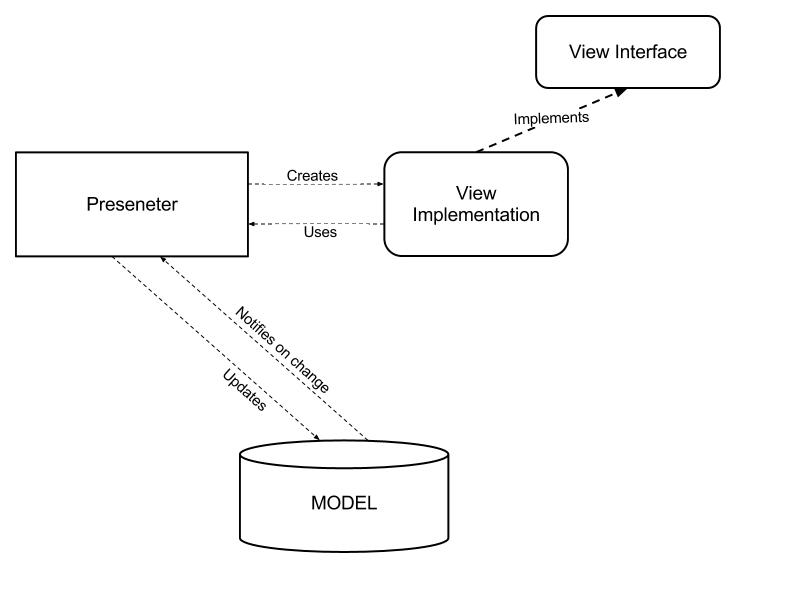
\includegraphics[width=\textwidth,
height=\textheight, keepaspectratio]{mvp.jpg}
	\caption{Model-View-Presenter}
	\label{fig:mvp}
\end{figure}
Advantages that Model-View-Presenter pattern offers are:
\begin{itemize}
  \item Clear design with completely separated handling of UI events form the actual handlers logic.
  \item Possibility to re-use interfaces of the views and presenters interfaces for different implementations.
  \item Separated test for the UI and for logic. 
\end{itemize}

\subsection{Presenter} Presenter exposes an interface that contains methods for all the actions that could be triggered in a view
like search, filtering, update etc. As an action is invoked by the view the presenter executes the necessary operation,
accessing model if needed. After that the presenter updates the view accordingly. Presenter is also responsible for
reaction on the changes of model not triggered by the current view.

\subsection{View} The view is logically clear composition of a set of user interface components that displays and/or gathers data
from the user. The view interface exposes all the methods that a presenter might need to assemble and steer it (e.g.
access to the parts of the view, getters/setters for some fields etc.). Ideally the view is not supposed to be bound to
any UI technology completely concealing its implementation from the presenter, so the presenter tells the view what to
do, whereas it is up to the view to decide how to do it. In case of Magnolia 5.0, however, we will break this rule and
for almost all the cases oblige the view to expose itself as a Vaadin component (because Vaadin is the only UI
technology used on the server-side).

\subsection{Model} Model is a data source used by a presenter. In Magnolia
CMS model is obviously a JCR repository. However, direct
access to JCR would be quite cumbersome and inefficient, so the actual communication with presenters in Magnolia 5.0
happens through the Vaadin data binding layer - a special JCR container, which will be discussed in the following chapter.

As it was already mentioned, MVP resembles Model-View-Controller pattern. However, in classic MVC the controller has to 
listen to both the View and the Model. This means, for instance, that the button click and text change handlers are registered
there. In MVP, on the other hand, the presenter only implmenets a set of certain functions that are invoked by the view.
Thus, MVP provides better decoupling between the view and the presentation. 

Besides already mentioned specialties of MVP use in Magnolia 5.0 (like a constraint to Vaadin) it is worth mentioning
that the main responsibilities are distributed differently than usual. Normally it is the job of the view to initialize
the presenter whereas in Magnolia 5.0 it is vice versa and the presenter creates the view. This difference is caused by
how the user interface is persisted in the back-end: JCR configuration repository contains only the information how to
build the UI which is a description of the presenter. Later when the user navigates to some specific view a pre-created
presenter instantiates the actual UI component.